\documentclass[12 pt]{article}
\usepackage{fancyhdr}
\usepackage[margin = 1 in]{geometry}
\usepackage{amsmath}
\usepackage{enumerate}
% \usepackage{indentfirst}
\pagestyle{fancy}
\usepackage{graphicx}
\usepackage[version=3]{mhchem}
\fancyhf{}
\usepackage{sectsty}	
\lhead{Andrew Wang}
\chead{CS/CNS/EE 155 Machine Learning \& Data Mining}
\rhead{Yue}
\sectionfont{\fontsize{15}{18}\selectfont}
\usepackage{graphicx}
\usepackage{array}
\newcolumntype{P}[1]{>{\centering\arraybackslash}p{#1}}
\newcolumntype{M}[1]{>{\centering\arraybackslash}m{#1}}
\usepackage[font=small,labelfont=bf]{caption}
\usepackage{float}
\usepackage{subfig}
\usepackage{microtype}
\usepackage{ amssymb }
\usepackage{amsmath}
\usepackage{commath}

\begin{document}
	\begin{center}
		\section*{Homework 2}
	\end{center}
	
	
	\subsection*{1 Comparing Different Loss Functions}	
	\noindent\textbf{Question A:} For classification, the squared error would excessively penalize outliers and hypothesis that yield high \textbf{w}$^T$x values will be severely penalized even if the \textbf{w}$^T$x values have the same sign as their respective y and thus classified correctly.\\
	
	\noindent\textbf{Question B:}  \\
	
	\begin{eqnarray*}
		\nabla_w L_{\text{hinge}} = \begin{cases} 
		0 & y\textbf{w}^T\textbf{x} \geq 1 \\
		-y\textbf{x} & y\textbf{w}^T\textbf{x} < 1 \\ 
		\end{cases}\\
		\end{eqnarray*} 
	\begin{eqnarray*}
		\nabla_w L_{\text{log}} = \frac{-\textbf{x}y}{e^{w^{T}xy} + 1}
	\end{eqnarray*}
	
		\begin{center}
			\begin{tabular}{c| c|c|c|c|c} 
				\hline
				x$_0$ & x$_1$ & x$_2$ & y & $\nabla_w$L$_{\text{hinge}}$  & $\nabla_w$L$_{\text{log}}$ \\ 
				\hline
				1 &0.5 & 3 & 1 & (-1,-0.5,-3) & (-0.378, -0.189, -1.133) \\ 
				1 &2 & -2 & 1 & (0,0,0) & (-0.119, -0.238, 0.238) \\
				1 &-3 & 1 & -1 & (0,0,0) & (0.047, -0.142, 0.047)\\
				\hline 
			\end{tabular}
		\end{center} 
	\noindent \newline The gradient of log loss will go to zero as \textbf{w}$^T$\textbf{x}y gets infinitely big meaning each prediction is a large positive number when y = 1 or a large negative number when y = -1, which makes sense given that minimizing log loss is the equivalent of maximizing likelihood. The gradient of hinge loss will converge to 0 when all the points are correctly classified because in this case, y\textbf{w}$^T$\textbf{x} $\geq$ 1 for all points. Thus, simply minimizing L$_\text{hinge}$ is not enough for "maximum margin" classification, because minimizing L$_\text{hinge}$ only ensures that points are classified correctly, but says nothing about margin. In order to maximize the margin, we must add the $\lambda\norm{w}^2$ term and minimize L$_\text{hinge}$ + $\lambda\norm{w}^2$ for accurate classification AND maximum margin. \\

	\noindent\textbf{Question C:} \noindent 
		\begin{figure}[H]
			\centering
			\subfloat{{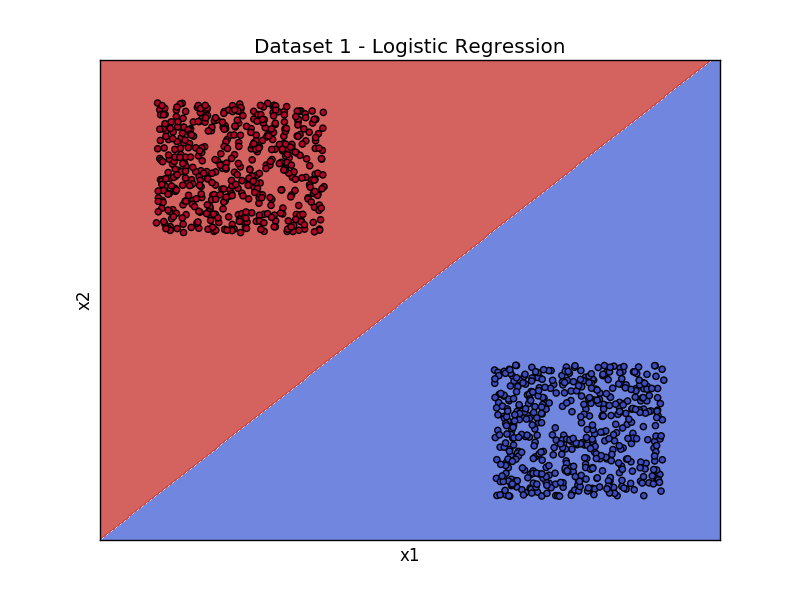
\includegraphics[width=8.5cm]{dataset1_log} }}%
			%\qquad
			\subfloat{{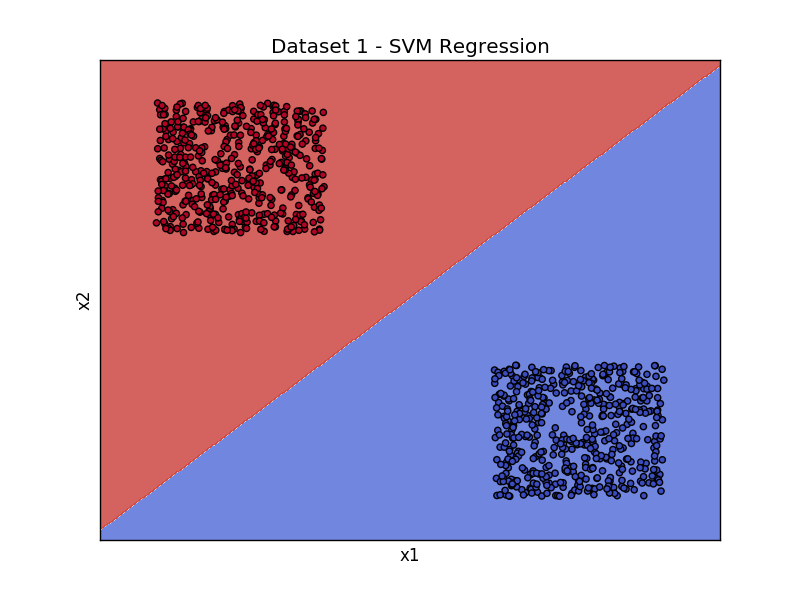
\includegraphics[width=8.5cm]{dataset1_SVM} }}%
		\end{figure}
		
		\begin{figure}[H]
			\centering
			\subfloat{{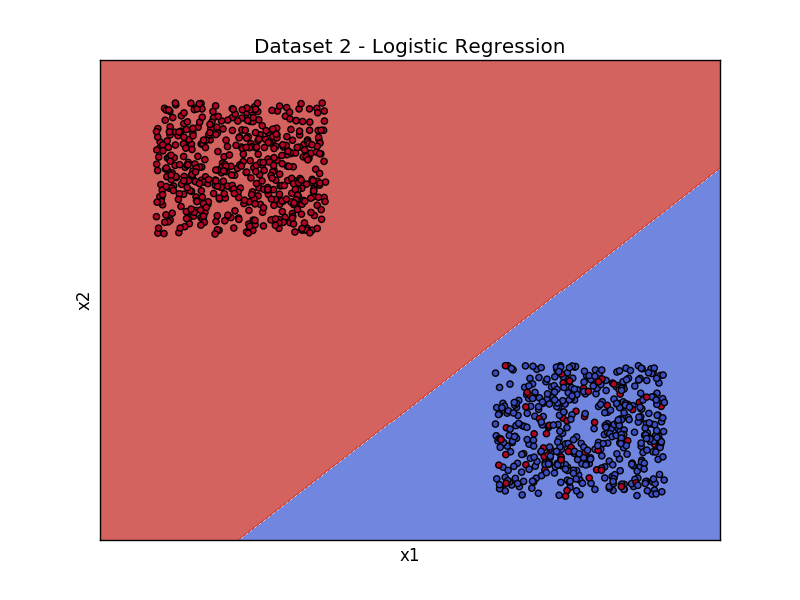
\includegraphics[width=8.5cm]{dataset2_log} }}%
			%\qquad
			\subfloat{{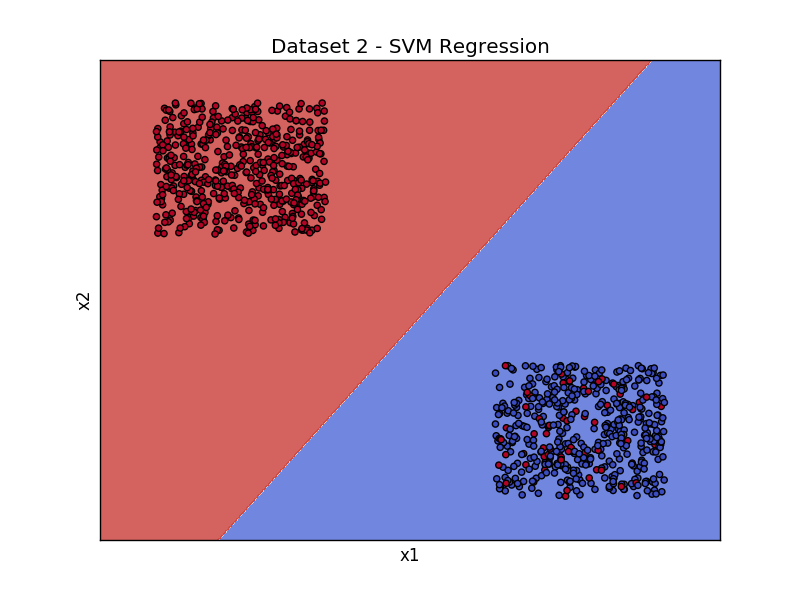
\includegraphics[width=8.5cm]{dataset2_SVM} }}%
		\end{figure}
		
		\begin{figure}[H]
			\centering
			\subfloat{{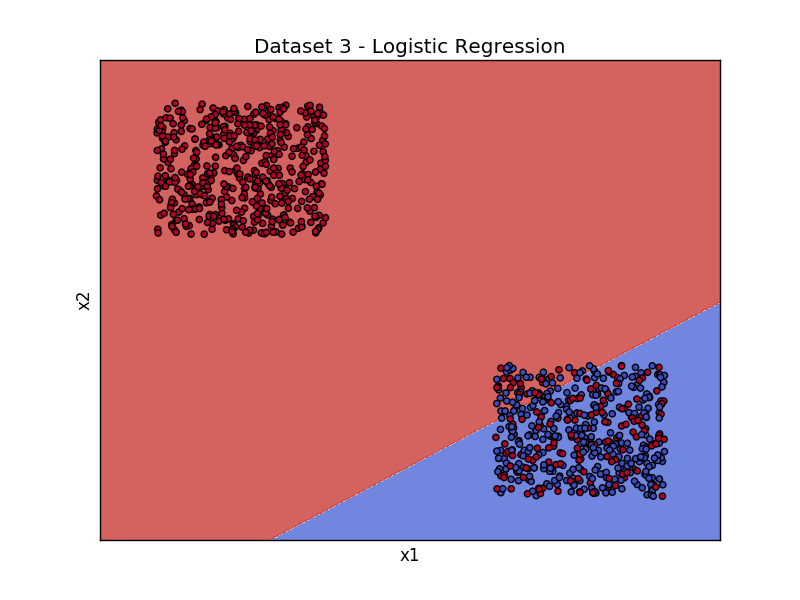
\includegraphics[width=8.5cm]{dataset3_log} }}%
			%\qquad
			\subfloat{{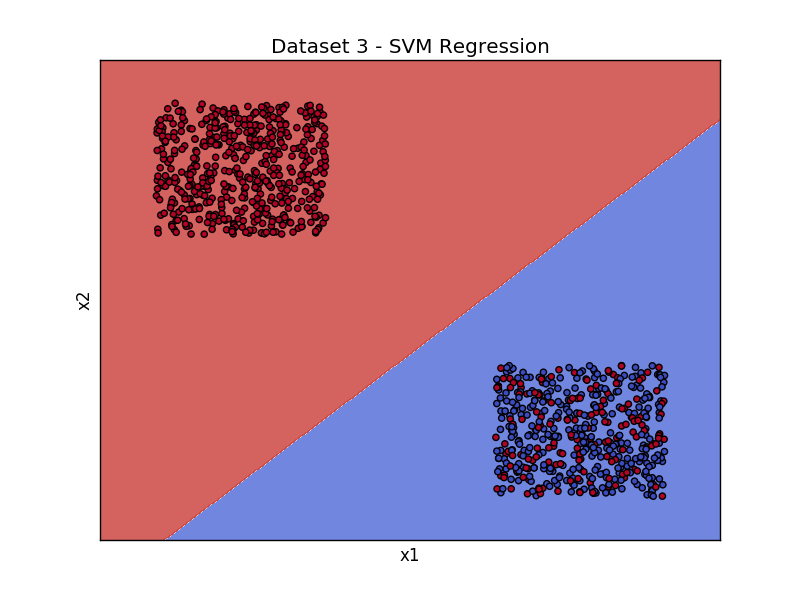
\includegraphics[width=8.5cm]{dataset3_SVM} }}%
		\end{figure}
		
		\noindent It appears that with more outliers, the logistic regression model has the boundary closer to the negatively labeled points. This makes sense because for the logistic regression model, the more noise, the more the boundary will be shifted to towards the errors to minimize the log error and thereby maximize likelihood. For the SVM however, we see a much more balanced or "even" divide between the two clusters and with increasing noise, the boundary shifts towards the negative cluster much less than the boundary shift of logistic regression with increasing noise. This makes sense given that because logistic regression is trying to maximize likelihood, it will shift the boundary farther towards the noisy cluster (even cutting through it in the case of 15\% noise) to maximize the probabilities of correct classification. However, the SVM does not shift its boundary nearly as much because it is worried about maximum margin and harsh penalties for misclassification. In the case of 15\% noise, unlike the logistic regression, the SVM does not cut through the data because in doing so would put it at risk of misclassifying more negative points than correctly classifying the positive points which are noise. \\
	
	\noindent\textbf{Question D:}  
		\begin{figure}[H]
			\centering
			\subfloat{{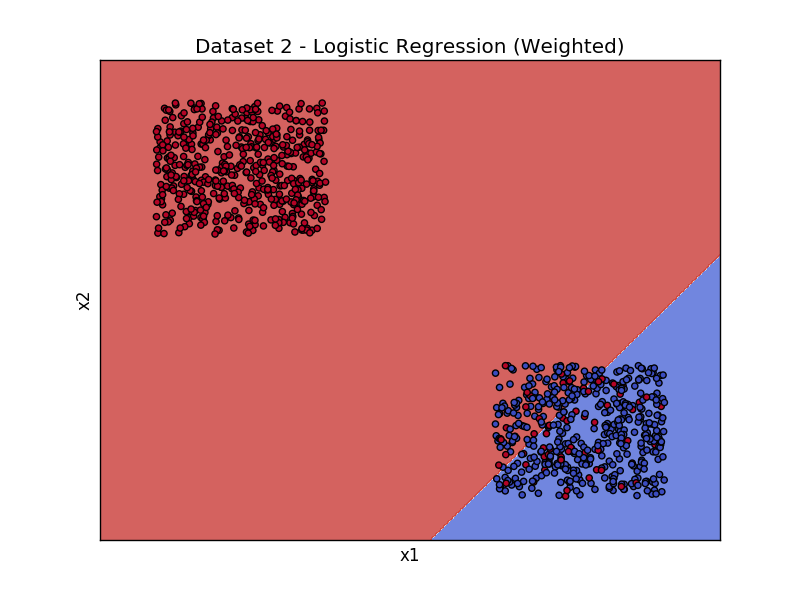
\includegraphics[width=8.5cm]{dataset2_log_weighted} }}%
			%\qquad
			\subfloat{{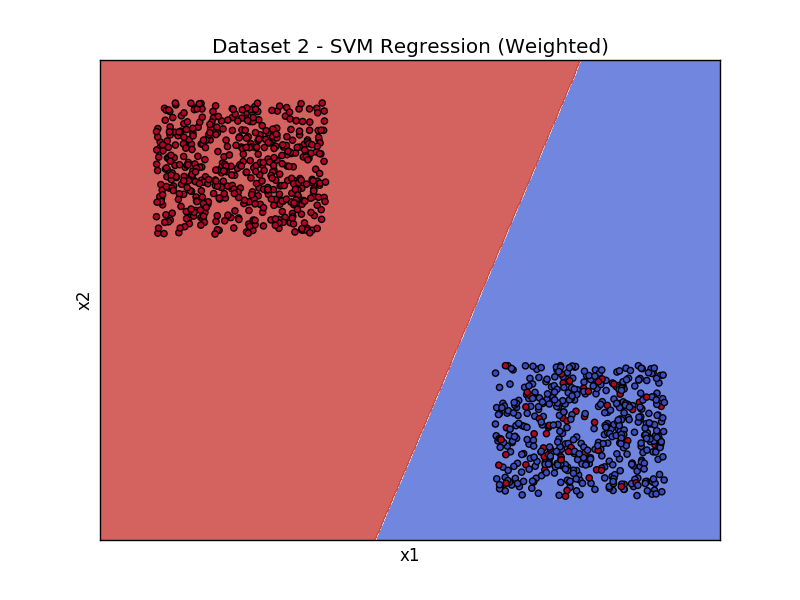
\includegraphics[width=8.5cm]{dataset2_SVM_weighted} }}%
		\end{figure}
	\noindent Both the logistic regression and SVM models shift towards the negative cluster which contains some noise meaning that there are some positive points in this cluster. This makes sense because now that positive points are weighed 5x that of negative points, the models now put more emphasis on correctly classifying the positive points in the negative cluster because with 5x the weight, the loss of not correctly classifying a positive point is much greater than that of misclassifying a negative point. Again, we see that the SVM regression's boundary is much more neutral than that of the logistic regression which can be attributed again to margin maximization and fear of misclassification.\\ 
 
	
	\subsection*{2 Effects of Regularization}
	\noindent\textbf{Question A:} No, adding the term cannot decrease the training error. For least-squares linear regression, the unregularized, closed-form solution, is the optimal solution for minimizing in-sample error. Adding a penalty form cannot further decrease the training error. Adding a penalty term will not always decrease the out-of-sample error either. When there is overfitting, regularization can improve generalization by reducing variance. However, if regularization is overused and we reduce variance by too much, bias will increase and we may be at risk for underfitting. So, although regularization can decrease out-of-sample errors, it may not always do so as it depends on the parameters of regularization. \\
	
	\noindent\textbf{Question B:} Unlike the $\ell_1$ norm, the $\ell_0$ norm is nonconvex and noncontinuous. This is problematic for minimization as derivatives/ gradients are necessary for the minimization of a regularized error. Thus, $\ell_0$ regularization is rarely used. \\
	
	\noindent\textbf{Question C:}  \\
	\begin{figure}[H]
	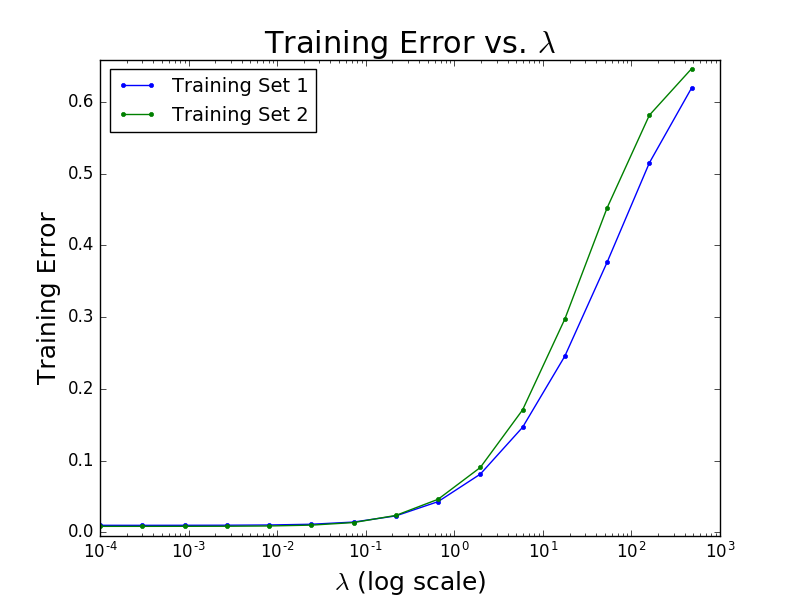
\includegraphics[width=12cm]{TrainingError2C}
	\end{figure}	

	\begin{figure}[H]
	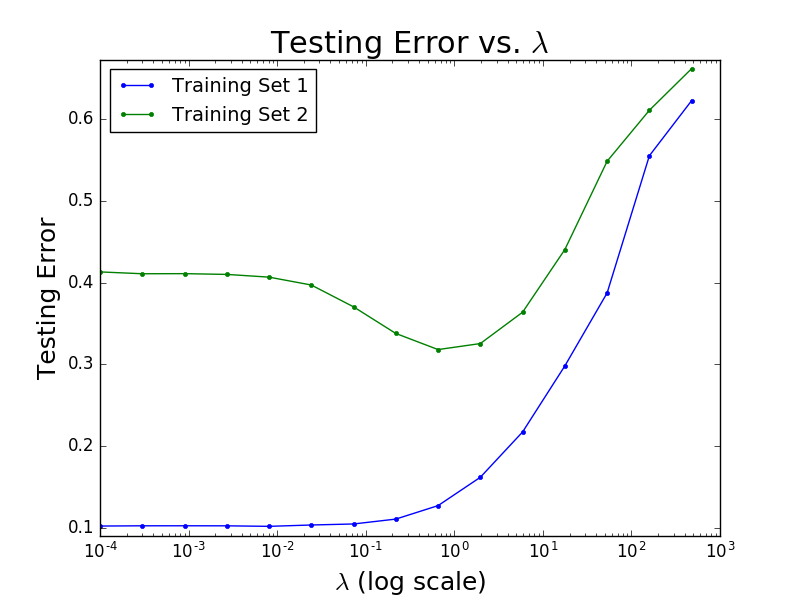
\includegraphics[width=12cm]{TestingError2C}
	\end{figure}

	\begin{figure}[H]
	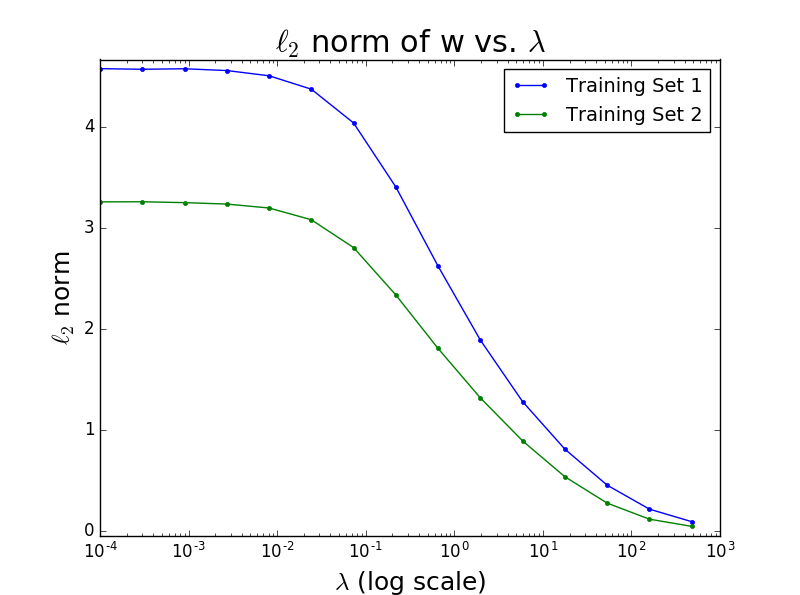
\includegraphics[width=12cm]{l2Norm}
	\end{figure}
	\noindent\textbf{Question D:} Given that second training set is a subset of the first training set and thereby contains fewer training points, we expect and observe the testing error resulting from training set 1 to be lower than that from training set 2 (more training examples decreases variance, bias about the same with constant $\lambda$, so thus testing error decreases). We see clear overfitting for set 2 with increasing testing error as $\lambda$ decreases for the first half of the graph while overfitting is not as clear for set 1, again confirming that variance decreases with increased training size. \\\\Regarding training error, training set 1 has a higher(ever so slightly) E$_\text{in}$ at lower $\lambda$ and lower E$_\text{in}$ at high $\lambda$, when compared to the training errors for training set 2. This can be attributed to the fact that because training set 2 is a subset of training set 1, at lower $\lambda$, complex models will be able to fit the dataset containing fewer points better, thus explaining why training set 1 has the higher E$_\text{in}$ for small $\lambda$. For large $\lambda$ and thus simpler models, points with larger error for the smaller dataset (training set 2) will negatively affect the E$_\text{in}$ of the smaller dataset more than the E$_\text{in}$ of the larger data set, thus why the training error for training set 1 is lower for large $\lambda$.\\
	
	\noindent\textbf{Question E:} There seems to be little overfitting.  Using Python, I found that out of the 15 points plotted, the minimum test error came on point 3, when $\lambda$ = 9.00 x 10$^{-3}$, but for the $\lambda$ values less than this, the testing error is only slightly bigger (hard to qualitatively tell from the graph as it appears that the testing error starts at the minimum from the first $\lambda$.) This contrasts with the testing error from fitting to set 2 where for the first half of the graph, we have increasing testing error with decreasing $\lambda$, a true sign of overfitting. However, in both cases, we do see underfitting. With increasing $\lambda$, especially after $\lambda$ = 1, the training and testing errors vastly increase, signaling that for these large $\lambda$, we are regularizing so much that the constrained model is too simple to capture the dataset accurately. \\
	
	\noindent\textbf{Question F:} We see that the $\ell_2$ norm of \textbf{w} decreases with increasing $\lambda$. This makes sense because with increasing $\lambda$, there is a greater emphasis on the regularization term of the $\ell_2$-regularized logistic error. \\
	
	\noindent\textbf{Question G:} Using Python, I found that the minimum testing error came from $\lambda$ = 0.6561. At this $\lambda$, we have the lowest E$_\text{out}$, meaning the best chance of generalizing out of sample.\\
	
	\subsection*{3 Lasso vs. Ridge Regularization}
	\noindent\textbf{Question A:} 
	\begin{figure}[H]
	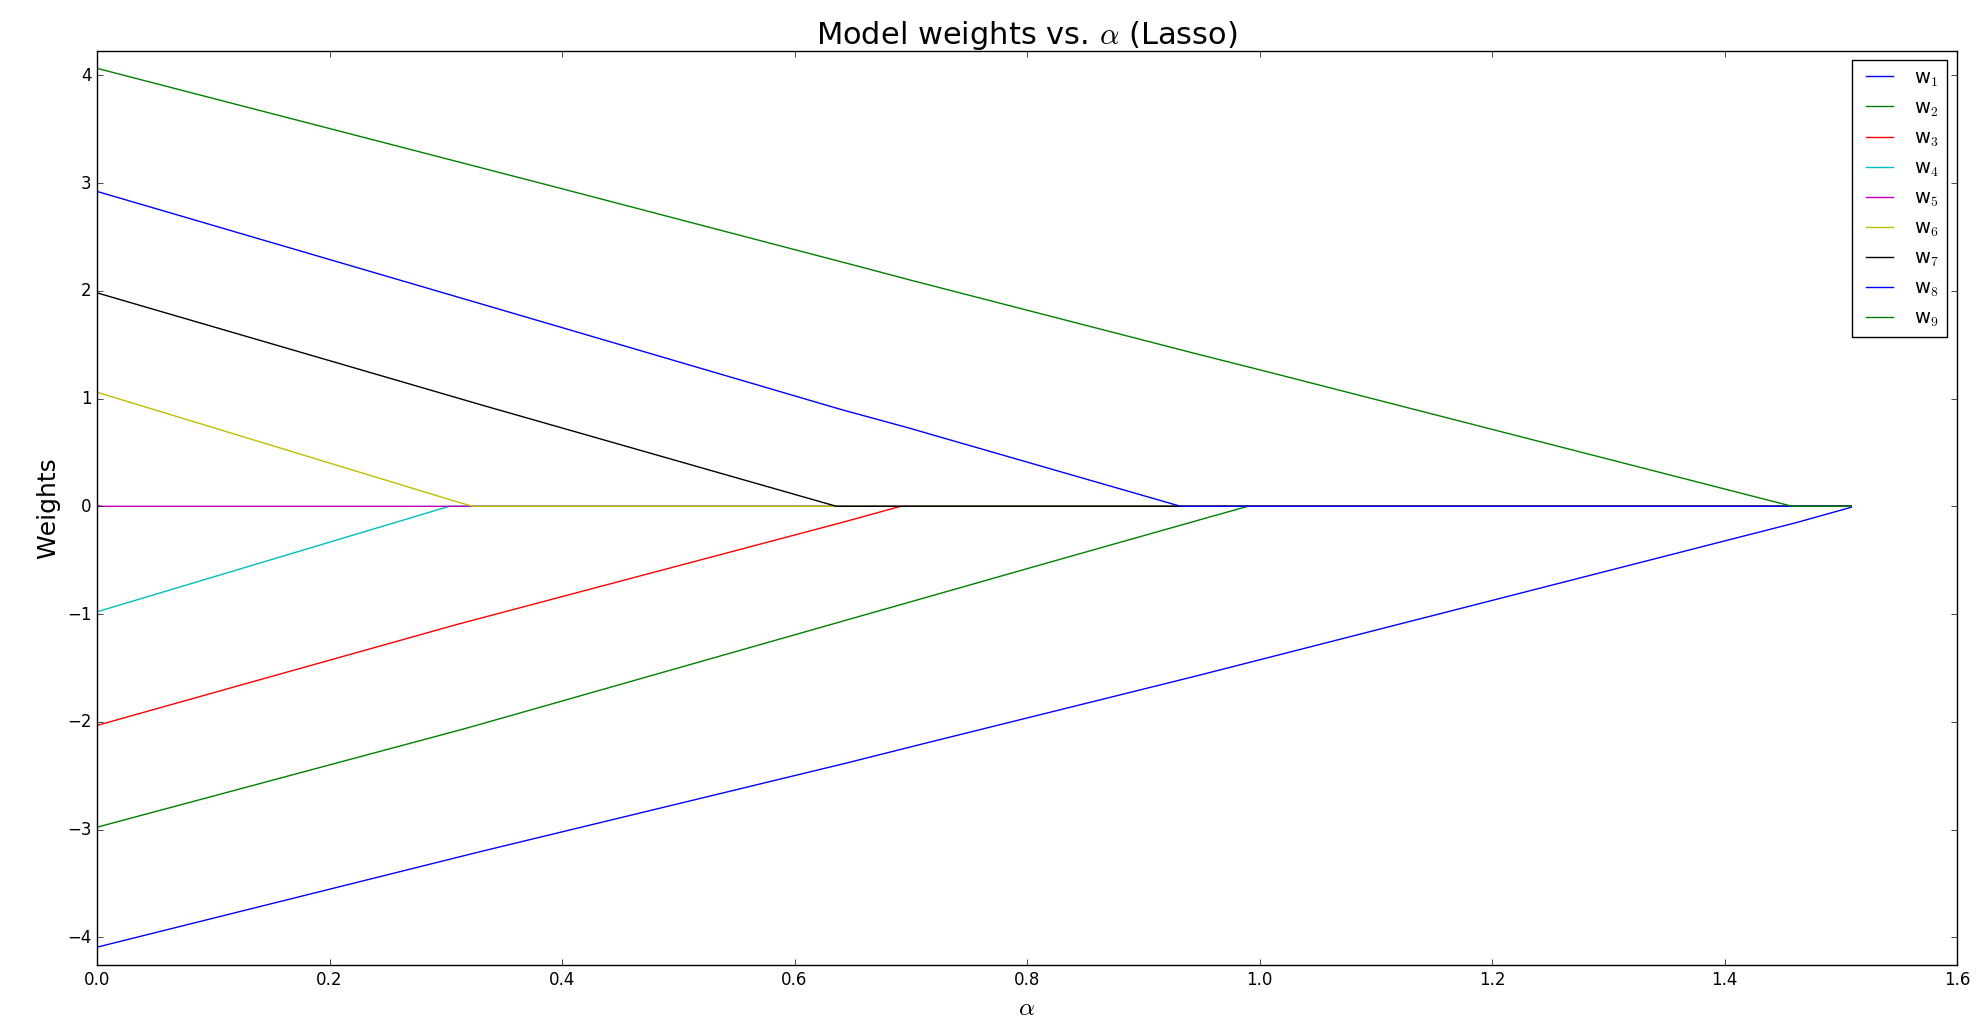
\includegraphics[width=14cm]{lasso_alpha}
	\end{figure}
	\begin{figure}[H]
	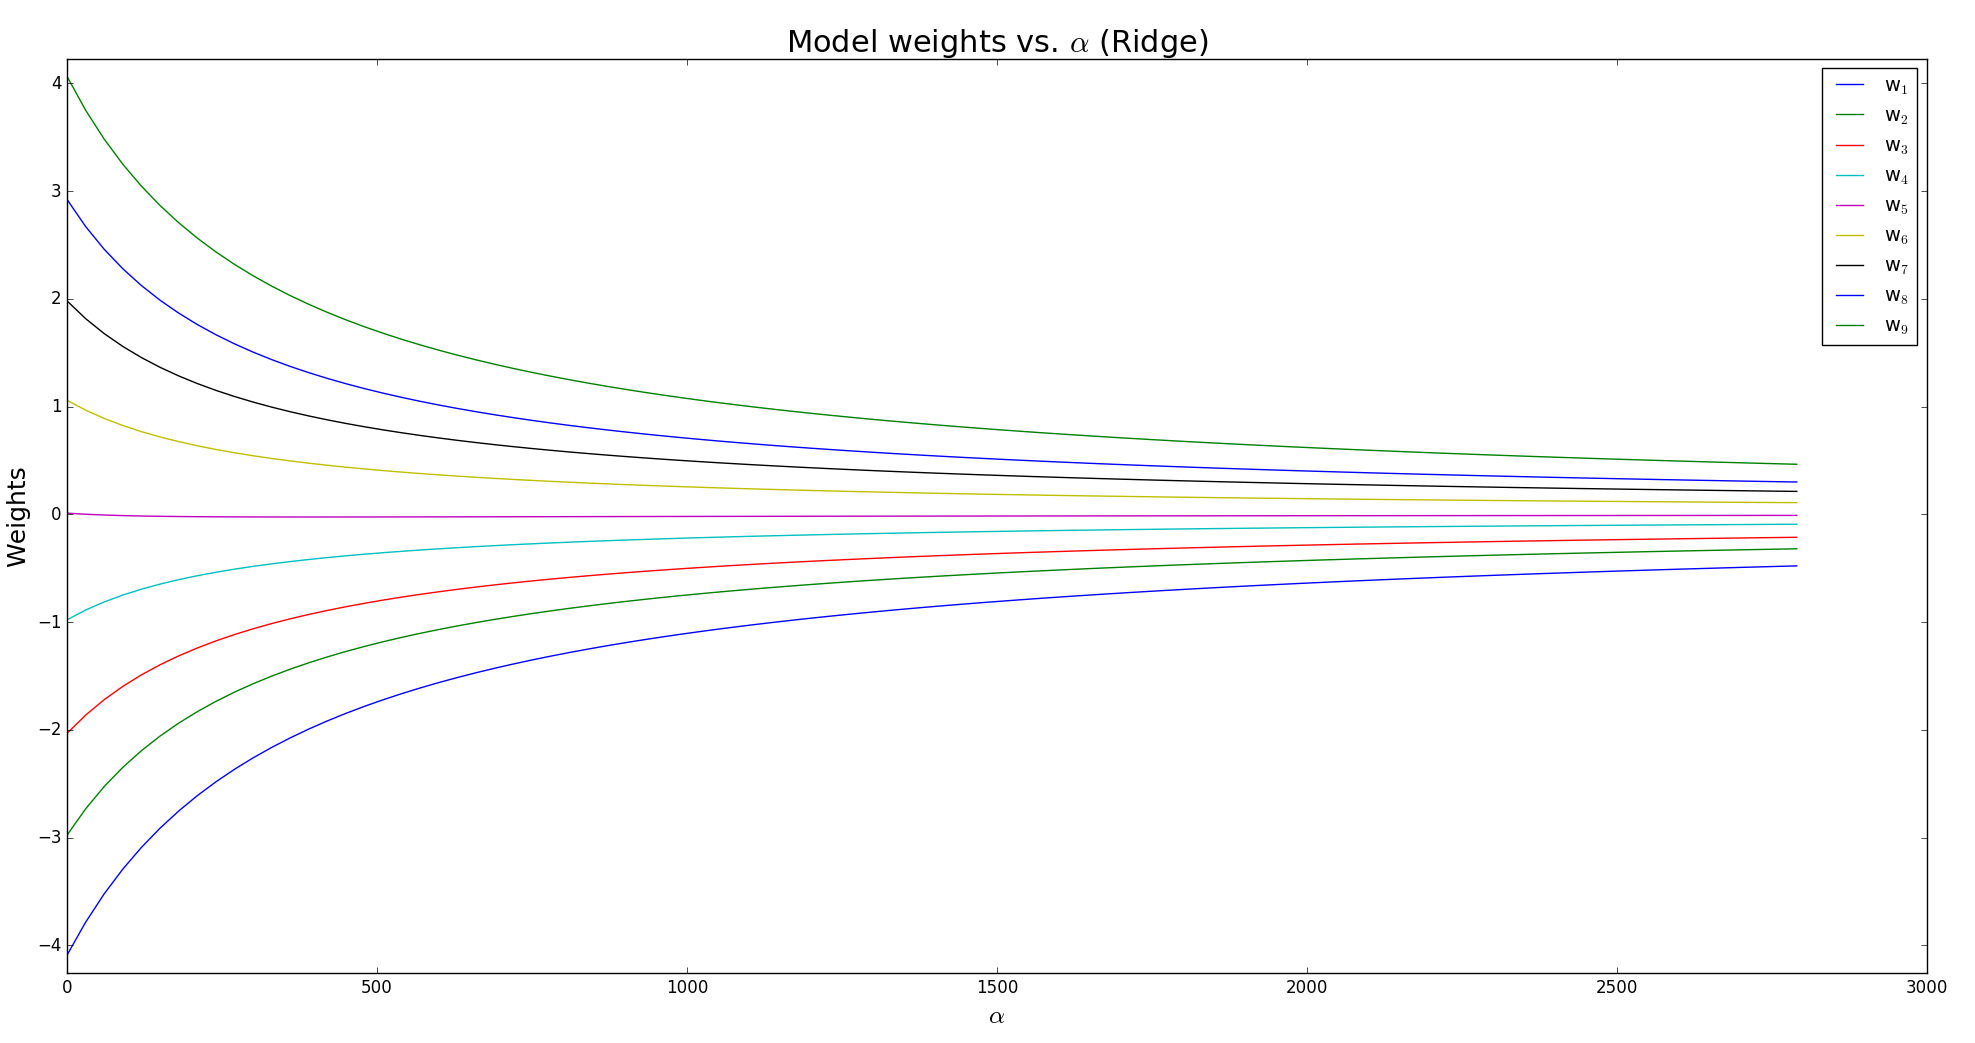
\includegraphics[width=14cm]{ridge_alpha}
	\end{figure}
	
	\noindent As the regularization parameter increases, the number of model weights that are exactly zero with lasso regression increase. For Ridge regression, the weights get closer and closer to zero, but none of the model weights actually become zero (asymptotic). \\ \\
	\noindent\textbf{Question B:} \\
	
	\noindent \textit{i.} We take the subgradient.
	\begin{eqnarray*}
		\nabla_{w_1} \Big[ \space{\norm{\textbf{y} - \textbf{X}^{T}\textbf{w}}^2 + \lambda\norm{\textbf{w}}_1}\Big] \\
		= -2\textbf{X}^T (\textbf{y} - \textbf{X}^{T}\textbf{w}) + \lambda = 0\\
		\rightarrow \textbf{w} = -(\lambda - 2 \textbf{X}^T\textbf{y}){(2\textbf{X}^T\textbf{X})}^{-1}
	\end{eqnarray*} 

	\noindent\textit{ii.} Yes, when $\lambda$ =  $\norm{2 \textbf{X}^T\textbf{y}}$, w$_1$ goes to 0. \\
	
	\noindent\textit{iii.}
	
	\begin{eqnarray*}
	\partial_w \Big[ \space{\norm{\textbf{y} - \textbf{X}^{T}\textbf{w}}^2 + \lambda\norm{\textbf{w}}_1}^2\Big] \\
	= -2\textbf{X}^T (\textbf{y} - \textbf{X}^{T}\textbf{w}) + 2\lambda\textbf{w} = 0 \\
	\rightarrow \textbf{w} = \textbf{X}^T\textbf{y}(\lambda I + \textbf{X}^T\textbf{X})^{-1}
	\end{eqnarray*} 
	\noindent\textit{iv.} No, there does not exist a $\lambda$ $>$ 0 such that w$_i$ = 0. \\
	
	\noindent Let's say, for the sake of argument, that $\textbf{w}$ = 0. Now, we multiply both sides by $\lambda I + \textbf{X}^T\textbf{X}$ (we know $\lambda$ $>$ 0) and get that 0 = $\textbf{X}^T\textbf{y}$ which clearly does not depend on $\lambda$. 
	This is consistent with our previous findings of Ridge regression, where weights get closer to 0, but never actually equal 0.\\
\end{document}